\documentclass[11pt]{article}

\usepackage[T1]{fontenc}
\usepackage[utf8]{inputenc}
\usepackage{lmodern}
\usepackage{amsmath,amssymb,amsthm,mathtools}
\usepackage{geometry}
\usepackage{graphicx}
\usepackage{hyperref}
\usepackage{enumitem}
\usepackage{booktabs}
\usepackage{longtable}
\usepackage{tikz}
\usetikzlibrary{arrows.meta,positioning,fit,backgrounds}

\geometry{margin=1in}
\setlist[itemize]{leftmargin=1.5em}
\setlist[enumerate]{leftmargin=1.75em}
\emergencystretch=3em

\newcommand{\ec}[1]{\texttt{\detokenize{#1}}}
\newcommand{\Fq}{\mathbf F_q}
\newcommand{\Z}{\mathbb Z}
\newcommand{\br}{\operatorname{br}_8}
\newcommand{\Rmont}{R}
\newcommand{\zroot}{\zeta}
\newcommand{\polyrepr}{\mathsf{poly\_repr\_bound}}
\newcommand{\fullntt}{\mathsf{FullNTT}}
\newcommand{\fullinvntt}{\mathsf{FullInvNTT}}
\newcommand{\hoare}[3]{\left\{#2\right\}\;#1\;\left\{#3\right\}}

\newtheorem{theorem}{Theorem}
\newtheorem{lemma}{Lemma}
\newtheorem{proposition}{Proposition}
\newtheorem{definition}{Definition}
\newtheorem{remark}{Remark}

\title{Full HAETAE Jasmin NTT Verification in EasyCrypt}
\author{Codex Proof Notes}
\date{29 April 2026}

\begin{document}
\maketitle

\begin{abstract}
This report records the completed machine-checked correctness proof for the
HAETAE NTT implementation extracted from Jasmin into EasyCrypt.  The final
EasyCrypt entry point is \ec{NTTEndToEnd.ec}.  It proves that the public
Jasmin wrapper \ec{Hpoly_extract.M.poly_ntt_jazz} computes the abstract
full polynomial NTT \ec{NTTFullSpec.full_ntt}, and that
\ec{Hpoly_extract.M.poly_invntt_jazz} computes the inverse abstract polynomial
NTT \ec{NTTFullSpec.full_invntt}, with the expected Montgomery-scaled output
representation for the inverse.  The proof chain is
\[
  \text{public Jasmin wrapper}
  \;\longrightarrow\;
  \text{Jasmin core}
  \;\longrightarrow\;
  \text{imperative EasyCrypt NTT core}
  \;\longrightarrow\;
  \text{closed-form abstract polynomial NTT}.
\]
The report also gives a file-by-file mathematical explanation of the remaining
\ec{.ec} files after cleanup.  Files moved to \ec{rubbish/} are scratch,
debug, or probe artifacts and are not part of the proof chain described here.
\end{abstract}

\tableofcontents

\section{Statement of the Verified Result}

\subsection{Mathematical domain}

The coefficient field is
\[
  \Fq = \Z/q\Z,
  \qquad q = 64513.
\]
In EasyCrypt, this is the type \ec{coeff} imported from \ec{GFq.ec}, and
polynomials are represented as arrays of exactly 256 coefficients:
\[
  \mathsf{poly} = \Fq^{256},
  \qquad
  \ec{type poly = coeff Array256.t}.
\]
The root used by the HAETAE NTT is
\[
  \zroot = \ec{zroot} = \ec{incoeff 426}.
\]
The bit-reversal permutation on eight bits is written
\[
  \br(i) = \ec{bsrev 8 i}.
\]

\begin{definition}[full forward transform]
For \(p\in\Fq^{256}\), the full forward transform proved in
\ec{NTTFullSpec.ec} is
\[
  \fullntt(p)_i
  =
  \sum_{j=0}^{255}
    p_j\,\zroot^{(2\br(i)+1)j},
  \qquad 0\le i<256.
\]
This is the operation \ec{NTTFullSpec.full_ntt}.
\end{definition}

\begin{definition}[full inverse transform]
For \(p\in\Fq^{256}\), the full inverse transform proved in
\ec{NTTFullSpec.ec} is
\[
  \fullinvntt(p)_i
  =
  \sum_{j=0}^{255}
    256^{-1}\,p_j\,
    \zroot^{-((2\br(j)+1)i)},
  \qquad 0\le i<256.
\]
This is the operation \ec{NTTFullSpec.full_invntt}.
\end{definition}

\subsection{Concrete representation relation}

The implementation works on \ec{BArray1024.t}, a 1024-byte array that stores
256 little-endian 32-bit words.  The main representation relation is
\[
  \ec{NTT_Fq.poly_repr_bound rp p b}.
\]
It means:
\begin{enumerate}
  \item for every index \(0\le i<256\), the 32-bit word stored at
        \(\ec{rp}[i]\) denotes the field element \(p_i\);
  \item the signed integer value of that word is bounded by \(2^b\), written in
        the development as \ec{Fq.bw32};
  \item the bound is strong enough to rule out the machine-word overflows used
        by the butterfly and Montgomery multiplication proofs.
\end{enumerate}

The output bound for the forward NTT is 24.  The output bound for the inverse
NTT is 16 after the final Montgomery scaling loop.

\subsection{Final machine-checked theorems}

\begin{theorem}[forward HAETAE Jasmin NTT correctness]
The theorem \ec{NTTEndToEnd.haetae_jasmin_ntt_correct} proves:
\[
\begin{aligned}
&\hoare{
  \ec{Hpoly_extract.M.poly_ntt_jazz}
}{
  \ec{NTT_Fq.poly_repr_bound rp p 16}
}{
  \ec{NTT_Fq.poly_repr_bound res (NTTFullSpec.full_ntt p) 24}
}.
\end{aligned}
\]
Thus the public Jasmin NTT wrapper returns a byte array representing the full
abstract polynomial NTT of the input polynomial.
\end{theorem}

\begin{theorem}[inverse HAETAE Jasmin NTT correctness]
The theorem \ec{NTTEndToEnd.haetae_jasmin_invntt_correct} proves:
\[
\begin{aligned}
&\hoare{
  \ec{Hpoly_extract.M.poly_invntt_jazz}
}{
  \ec{NTT_Fq.poly_repr_bound rp p 16}
}{
  \ec{NTT_Fq.poly_repr_bound res}
  \bigl(\ec{NTT_Fq.array256_mont (NTTFullSpec.full_invntt p)}\bigr)
  \ec{16}
}.
\end{aligned}
\]
The inverse implementation therefore returns the Montgomery-scaled
representation of the abstract inverse transform.  This scaling is intentional:
it is the postcondition delivered by the extracted Jasmin inverse core after
its final multiplication by the inverse table entry at index 255.
\end{theorem}

\begin{remark}
The theorem is an implementation-correctness theorem for the HAETAE NTT
routines, not for the entire HAETAE signature scheme.  It is relative to the
EasyCrypt model of the extracted Jasmin procedures, the field and Montgomery
libraries imported by the proof, and the local representation relation.
\end{remark}

\section{Overall Proof Architecture}

The proof is organized as four mathematical bridges.

\begin{enumerate}
  \item \textbf{Public wrapper bridge.}
        \ec{RefJasminNTT.poly_ntt_jazz_ref} and
        \ec{RefJasminNTT.poly_invntt_jazz_ref} show that the public wrappers
        call exactly the corresponding internal cores.

  \item \textbf{Core pRHL bridge.}
        \ec{RefJasminNTT.poly_ntt_core_ref} and
        \ec{RefJasminNTT.poly_invntt_core_ref} relate the extracted Jasmin
        cores to the imperative EasyCrypt procedures
        \ec{NTT_Fq.NTT.ntt} and \ec{NTT_Fq.NTT.invntt}.  This is where
        machine-word bounds, table interpretations, Montgomery multiplication,
        and pRHL loop synchronization are proved.

  \item \textbf{Loop algebra bridge.}
        \ec{NTTFullAlgebra.ntt_full_ntt} and
        \ec{NTTFullAlgebra.invntt_full_invntt} prove that the imperative
        EasyCrypt procedures compute the closed-form polynomial transforms in
        \ec{NTTFullSpec.ec}.

  \item \textbf{End-to-end composition.}
        \ec{NTTEndToEnd.ec} composes the previous bridges and states the
        final public-entry-point Hoare triples.
\end{enumerate}

\begin{figure}[p]
\centering
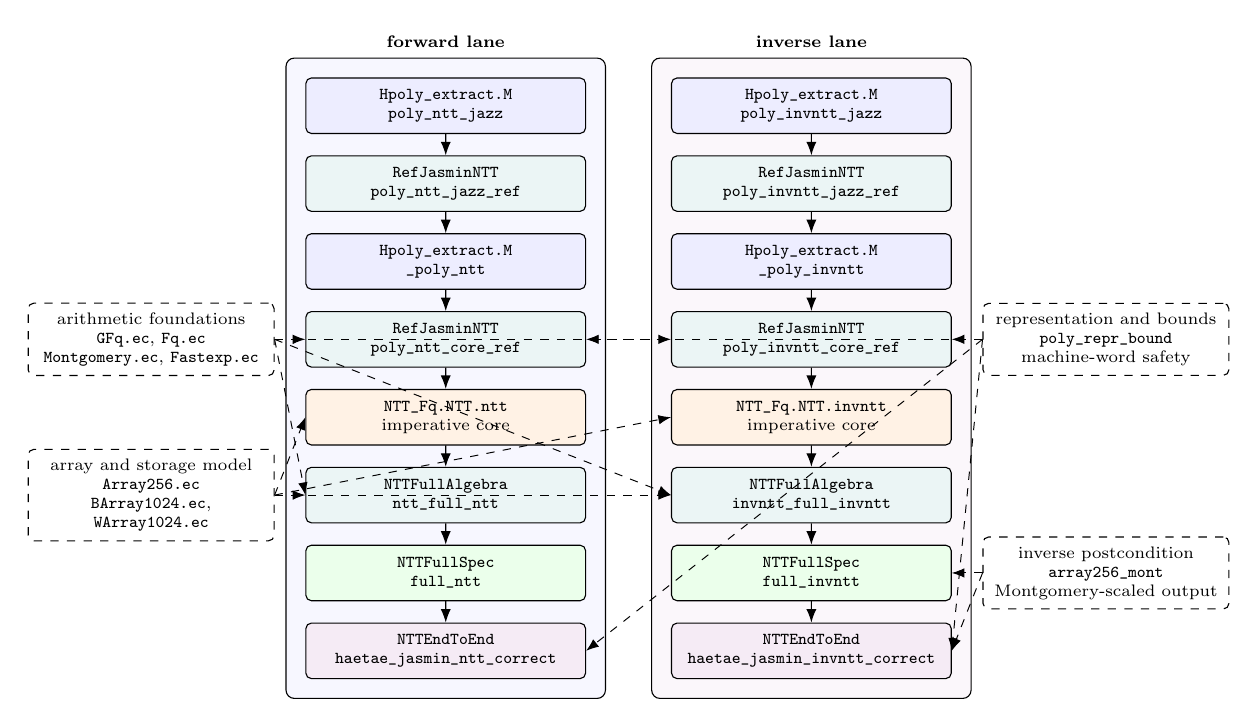
\begin{tikzpicture}[
  scale=0.86,
  transform shape,
  >=Latex,
  proofnode/.style={
    draw,
    rounded corners=2pt,
    align=center,
    inner sep=4pt,
    font=\scriptsize,
    text width=3.85cm,
    minimum height=0.82cm
  },
  public/.style={proofnode, fill=blue!7},
  bridge/.style={proofnode, fill=teal!8},
  core/.style={proofnode, fill=orange!10},
  spec/.style={proofnode, fill=green!8},
  final/.style={proofnode, fill=violet!8},
  support/.style={
    draw,
    dashed,
    rounded corners=2pt,
    align=center,
    inner sep=4pt,
    font=\scriptsize,
    text width=3.35cm,
    minimum height=0.78cm
  },
  arrow/.style={->, line width=0.42pt},
  supportarrow/.style={->, dashed, line width=0.35pt},
  grouplabel/.style={font=\scriptsize\bfseries, align=center}
]
  \node[grouplabel] at (0,0.95) {forward lane};
  \node[grouplabel] at (5.4,0.95) {inverse lane};

  \node[public] (pubf) at (0,0)
    {\ec{Hpoly_extract.M}\\ \ec{poly_ntt_jazz}};
  \node[public] (pubi) at (5.4,0)
    {\ec{Hpoly_extract.M}\\ \ec{poly_invntt_jazz}};

  \node[bridge] (wrapf) at (0,-1.15)
    {\ec{RefJasminNTT}\\ \ec{poly_ntt_jazz_ref}};
  \node[bridge] (wrapi) at (5.4,-1.15)
    {\ec{RefJasminNTT}\\ \ec{poly_invntt_jazz_ref}};

  \node[public] (coref) at (0,-2.3)
    {\ec{Hpoly_extract.M}\\ \ec{_poly_ntt}};
  \node[public] (corei) at (5.4,-2.3)
    {\ec{Hpoly_extract.M}\\ \ec{_poly_invntt}};

  \node[bridge] (prhlf) at (0,-3.45)
    {\ec{RefJasminNTT}\\ \ec{poly_ntt_core_ref}};
  \node[bridge] (prhli) at (5.4,-3.45)
    {\ec{RefJasminNTT}\\ \ec{poly_invntt_core_ref}};

  \node[core] (reff) at (0,-4.6)
    {\ec{NTT_Fq.NTT.ntt}\\ imperative core};
  \node[core] (refi) at (5.4,-4.6)
    {\ec{NTT_Fq.NTT.invntt}\\ imperative core};

  \node[bridge] (algf) at (0,-5.75)
    {\ec{NTTFullAlgebra}\\ \ec{ntt_full_ntt}};
  \node[bridge] (algi) at (5.4,-5.75)
    {\ec{NTTFullAlgebra}\\ \ec{invntt_full_invntt}};

  \node[spec] (specf) at (0,-6.9)
    {\ec{NTTFullSpec}\\ \ec{full_ntt}};
  \node[spec] (speci) at (5.4,-6.9)
    {\ec{NTTFullSpec}\\ \ec{full_invntt}};

  \node[final] (endf) at (0,-8.05)
    {\ec{NTTEndToEnd}\\ \ec{haetae_jasmin_ntt_correct}};
  \node[final] (endi) at (5.4,-8.05)
    {\ec{NTTEndToEnd}\\ \ec{haetae_jasmin_invntt_correct}};

  \node[support] (arith) at (-4.35,-3.45)
    {arithmetic foundations\\
     \ec{GFq.ec}, \ec{Fq.ec}\\
     \ec{Montgomery.ec}, \ec{Fastexp.ec}};
  \node[support] (arrays) at (-4.35,-5.75)
    {array and storage model\\
     \ec{Array256.ec}\\
     \ec{BArray1024.ec}, \ec{WArray1024.ec}};
  \node[support] (repr) at (9.75,-3.45)
    {representation and bounds\\
     \ec{poly_repr_bound}\\
     machine-word safety};
  \node[support] (inversepost) at (9.75,-6.9)
    {inverse postcondition\\
     \ec{array256_mont}\\
     Montgomery-scaled output};

  \draw[arrow] (pubf) -- (wrapf);
  \draw[arrow] (wrapf) -- (coref);
  \draw[arrow] (coref) -- (prhlf);
  \draw[arrow] (prhlf) -- (reff);
  \draw[arrow] (reff) -- (algf);
  \draw[arrow] (algf) -- (specf);
  \draw[arrow] (specf) -- (endf);

  \draw[arrow] (pubi) -- (wrapi);
  \draw[arrow] (wrapi) -- (corei);
  \draw[arrow] (corei) -- (prhli);
  \draw[arrow] (prhli) -- (refi);
  \draw[arrow] (refi) -- (algi);
  \draw[arrow] (algi) -- (speci);
  \draw[arrow] (speci) -- (endi);

  \draw[supportarrow] (arith.east) -- (prhlf.west);
  \draw[supportarrow] (arith.east) -- (prhli.west);
  \draw[supportarrow] (arith.east) -- (algf.west);
  \draw[supportarrow] (arith.east) -- (algi.west);
  \draw[supportarrow] (arrays.east) -- (reff.west);
  \draw[supportarrow] (arrays.east) -- (refi.west);
  \draw[supportarrow] (arrays.east) -- (algf.west);
  \draw[supportarrow] (arrays.east) -- (algi.west);
  \draw[supportarrow] (repr.west) -- (prhlf.east);
  \draw[supportarrow] (repr.west) -- (prhli.east);
  \draw[supportarrow] (repr.west) -- (endf.east);
  \draw[supportarrow] (repr.west) -- (endi.east);
  \draw[supportarrow] (inversepost.west) -- (speci.east);
  \draw[supportarrow] (inversepost.west) -- (endi.east);

  \begin{scope}[on background layer]
    \node[
      draw,
      rounded corners=3pt,
      fill=blue!3,
      fit=(pubf) (wrapf) (coref) (prhlf) (reff) (algf) (specf) (endf),
      inner sep=7pt
    ] {};
    \node[
      draw,
      rounded corners=3pt,
      fill=violet!3,
      fit=(pubi) (wrapi) (corei) (prhli) (refi) (algi) (speci) (endi),
      inner sep=7pt
    ] {};
  \end{scope}
\end{tikzpicture}
\caption{Structural proof script diagram for the full HAETAE NTT
verification.  Solid arrows are theorem-composition steps.  Dashed arrows mark
mathematical infrastructure used to discharge proof obligations, especially
field arithmetic, Montgomery reduction, array extensionality, representation
bounds, and the inverse Montgomery-scaled postcondition.}
\label{fig:haetae-ntt-proof-structure}
\end{figure}

\section{File-by-File Mathematical Map}

This section explains the mathematical content of every remaining \ec{.ec}
file in the cleaned verification directory.  The files in \ec{rubbish/} are
not included because they are no longer part of the proof target.

\begin{longtable}{p{0.25\linewidth}p{0.68\linewidth}}
\toprule
\textbf{File} & \textbf{Mathematical role in the proof} \\
\midrule
\endfirsthead
\toprule
\textbf{File} & \textbf{Mathematical role in the proof} \\
\midrule
\endhead
\ec{Array256.ec} &
Defines the length-256 coefficient array by cloning Jasmin's
\ec{PolyArray}.  It supplies finite-array extensionality, initialization,
lookup, and update principles used throughout the polynomial proofs. \\
\ec{BArray1024.ec} &
Defines 1024-byte arrays by cloning Jasmin's byte-array theory.  This is the
concrete storage type for 256 32-bit coefficients. \\
\ec{WArray1024.ec} &
Defines 1024-word arrays by cloning Jasmin's word-array theory.  It is a
support artifact of the extracted Jasmin memory model. \\
\ec{extract/Array256.ec},
\ec{extract/BArray1024.ec},
\ec{extract/WArray1024.ec} &
Generated extraction-side counterparts of the array theories.  They document
and support the original extraction environment; the main proof imports the
top-level copies. \\
\ec{GFq.ec} &
Introduces the finite field modulus \(q=64513\), assumes its primality, and
defines signed representatives, compression, and decompression. \\
\ec{Rq.ec} &
Defines polynomials over \(\Fq\), ring operations, an older split even/odd
\ec{Rq.ntt}, \ec{Rq.invntt}, and base multiplication.  The report explains why
\ec{Rq.ntt} is not the full 256-point HAETAE NTT. \\
\ec{Montgomery.ec} &
Provides generic signed and classical Montgomery-reduction mathematics:
division facts, signed modular representatives, and REDC congruence/bound
theorems. \\
\ec{Fastexp.ec} &
Imports and instantiates exponentiation support used to reason about powers of
\(\zroot\), root orders, and bit-reversal exponents. \\
\ec{Fq.ec} &
Proves correctness and losslessness of the extracted Jasmin field routines
\ec{__montgomery_reduce} and \ec{__fqmul}. \\
\ec{Hpoly_extract.ec} &
Contains the extracted Jasmin procedures and concrete twiddle tables
\ec{jzetas} and \ec{jzetas_inv}.  The NTT proof reasons about
\ec{_poly_ntt}, \ec{_poly_invntt}, \ec{poly_ntt_jazz}, and
\ec{poly_invntt_jazz}. \\
\ec{extract/Hpoly_extract.ec} &
Generated extraction artifact containing the same procedures and generated
wrapper lemmas.  The main proof uses the top-level \ec{Hpoly_extract.ec} plus
locally proved wrapper equivalences. \\
\ec{NTT_Fq.ec} &
Defines the imperative EasyCrypt NTT and inverse NTT procedures, the abstract
twiddle arrays, Montgomery table interpretation, and the byte-array
representation relation. \\
\ec{NTTFullSpec.ec} &
Defines the closed-form full forward and inverse NTT specifications and proves
that the bit-reversed loop specification implies the closed-form formulas. \\
\ec{NTTFullAlgebra.ec} &
Contains the main loop-level mathematical proof that
\ec{NTT_Fq.NTT.ntt} and \ec{NTT_Fq.NTT.invntt} compute
\ec{NTTFullSpec.full_ntt} and \ec{NTTFullSpec.full_invntt}. \\
\ec{RefJasminNTT.ec} &
Contains the pRHL proof connecting extracted Jasmin cores to the imperative
EasyCrypt NTT cores, including machine-word bounds, Montgomery multiplication,
twiddle-table cancellation, and wrapper equivalences. \\
\ec{NTTEndToEnd.ec} &
Composes all previous propositions into the final public-entry-point
implementation-correctness theorems. \\
\bottomrule
\end{longtable}

\section{Detailed Proof Inventory and File Structure}

This section records, file by file, what is actually proved in the
EasyCrypt development and how each group of propositions enters the final
claim.  Files whose only content is a clone or generated procedure body still
matter: they introduce semantic objects, array theories, or Jasmin procedures
that later files prove correct.

\begin{figure}[p]
\centering
\resizebox{\textwidth}{!}{%
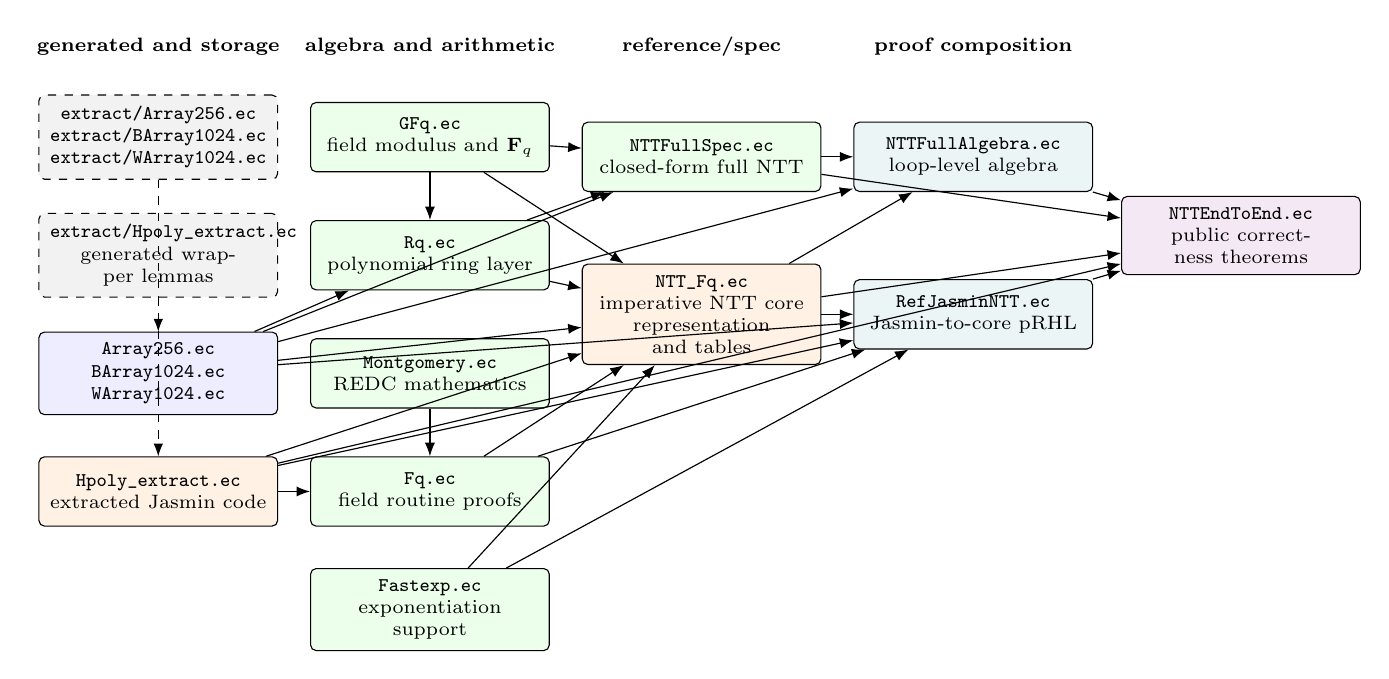
\begin{tikzpicture}[
  >=Latex,
  filenode/.style={
    draw,
    rounded corners=2pt,
    align=center,
    inner sep=4pt,
    font=\scriptsize,
    text width=2.75cm,
    minimum height=0.88cm
  },
  generated/.style={filenode, fill=gray!10, dashed},
  storage/.style={filenode, fill=blue!7},
  mathfile/.style={filenode, fill=green!8},
  implfile/.style={filenode, fill=orange!10},
  prooffile/.style={filenode, fill=teal!8},
  finalfile/.style={filenode, fill=violet!9},
  edge/.style={->, line width=0.42pt},
  softedge/.style={->, dashed, line width=0.35pt},
  label/.style={font=\scriptsize\bfseries}
]
  \node[label] at (-4.8,2.6) {generated and storage};
  \node[label] at (-1.35,2.6) {algebra and arithmetic};
  \node[label] at (2.1,2.6) {reference/spec};
  \node[label] at (5.55,2.6) {proof composition};

  \node[generated] (exarr) at (-4.8,1.45)
    {\ec{extract/Array256.ec}\\
     \ec{extract/BArray1024.ec}\\
     \ec{extract/WArray1024.ec}};
  \node[generated] (exhpoly) at (-4.8,-0.05)
    {\ec{extract/Hpoly_extract.ec}\\ generated wrapper lemmas};
  \node[storage] (arr) at (-4.8,-1.55)
    {\ec{Array256.ec}\\
     \ec{BArray1024.ec}\\
     \ec{WArray1024.ec}};
  \node[implfile] (hpoly) at (-4.8,-3.05)
    {\ec{Hpoly_extract.ec}\\ extracted Jasmin code};

  \node[mathfile] (gfq) at (-1.35,1.45)
    {\ec{GFq.ec}\\ field modulus and \(\Fq\)};
  \node[mathfile] (rq) at (-1.35,-0.05)
    {\ec{Rq.ec}\\ polynomial ring layer};
  \node[mathfile] (mont) at (-1.35,-1.55)
    {\ec{Montgomery.ec}\\ REDC mathematics};
  \node[mathfile] (fq) at (-1.35,-3.05)
    {\ec{Fq.ec}\\ field routine proofs};
  \node[mathfile] (fastexp) at (-1.35,-4.55)
    {\ec{Fastexp.ec}\\ exponentiation support};

  \node[implfile] (nttfq) at (2.1,-0.8)
    {\ec{NTT_Fq.ec}\\ imperative NTT core\\ representation and tables};
  \node[mathfile] (spec) at (2.1,1.2)
    {\ec{NTTFullSpec.ec}\\ closed-form full NTT};

  \node[prooffile] (alg) at (5.55,1.2)
    {\ec{NTTFullAlgebra.ec}\\ loop-level algebra};
  \node[prooffile] (refjas) at (5.55,-0.8)
    {\ec{RefJasminNTT.ec}\\ Jasmin-to-core pRHL};
  \node[finalfile] (end) at (8.95,0.2)
    {\ec{NTTEndToEnd.ec}\\ public correctness theorems};

  \draw[softedge] (exarr) -- (arr);
  \draw[softedge] (exhpoly) -- (hpoly);
  \draw[edge] (arr) -- (rq);
  \draw[edge] (arr) -- (nttfq);
  \draw[edge] (arr) -- (spec);
  \draw[edge] (arr) -- (alg);
  \draw[edge] (arr) -- (refjas);
  \draw[edge] (hpoly) -- (fq);
  \draw[edge] (hpoly) -- (nttfq);
  \draw[edge] (hpoly) -- (refjas);
  \draw[edge] (hpoly) -- (end);

  \draw[edge] (gfq) -- (rq);
  \draw[edge] (gfq) -- (nttfq);
  \draw[edge] (gfq) -- (spec);
  \draw[edge] (rq) -- (spec);
  \draw[edge] (rq) -- (nttfq);
  \draw[edge] (mont) -- (fq);
  \draw[edge] (fq) -- (nttfq);
  \draw[edge] (fq) -- (refjas);
  \draw[edge] (fastexp) -- (nttfq);
  \draw[edge] (fastexp) -- (refjas);

  \draw[edge] (nttfq) -- (alg);
  \draw[edge] (spec) -- (alg);
  \draw[edge] (nttfq) -- (refjas);
  \draw[edge] (alg) -- (end);
  \draw[edge] (refjas) -- (end);
  \draw[edge] (spec) -- (end);
  \draw[edge] (nttfq) -- (end);
\end{tikzpicture}%
}
\caption{File-structure diagram for the verification.  Solid arrows indicate
imports or theorem dependencies used by later proof files.  Dashed arrows show
the generated extraction copies that supply the original extraction context but
are not the main hand-written proof entry points.}
\label{fig:haetae-ntt-file-structure}
\end{figure}

\begingroup
\small
\begin{longtable}{p{0.20\linewidth}p{0.39\linewidth}p{0.34\linewidth}}
\toprule
\textbf{File} & \textbf{Proofs or propositions contained in the file} &
\textbf{Role in the final theorem} \\
\midrule
\endfirsthead
\toprule
\textbf{File} & \textbf{Proofs or propositions contained in the file} &
\textbf{Role in the final theorem} \\
\midrule
\endhead
\ec{Array256.ec} &
No hand-written lemmas are added.  The file clones Jasmin's
\ec{PolyArray} at size 256, thereby importing the full finite-array proof
theory: lookup after initialization, lookup after update, update
extensionality, and equality by pointwise equality. &
All polynomial specifications and loop invariants are stated over
\ec{Array256.t}.  The update and extensionality facts are used in
\ec{NTTFullSpec.ec}, \ec{NTTFullAlgebra.ec}, \ec{NTT_Fq.ec}, and
\ec{RefJasminNTT.ec}. \\

\ec{BArray1024.ec} &
No local NTT proof is added.  The file clones Jasmin's byte-array theory at
size 1024.  The imported propositions give reads and writes over the concrete
byte memory used to store 256 little-endian 32-bit coefficients. &
It is the concrete carrier of the public Jasmin input and output arrays.  The
representation predicates in \ec{NTT_Fq.ec} and the pRHL proof in
\ec{RefJasminNTT.ec} rely on its byte-level update theory. \\

\ec{WArray1024.ec} &
No local NTT proof is added.  The file clones Jasmin's word-array theory at
size 1024. &
It supports the extracted Jasmin memory model and keeps the extraction
environment coherent with Jasmin's word-array libraries. \\

\ec{extract/Array256.ec} &
Generated clone of the extraction-side 256-element array theory.  It contains
no hand-written NTT correctness proof. &
Records the original extraction context.  The cleaned proof uses the top-level
\ec{Array256.ec} as the imported array theory. \\

\ec{extract/BArray1024.ec} &
Generated clone of the extraction-side 1024-byte array theory. &
Records the original extraction context for byte arrays.  The active proof
imports the top-level \ec{BArray1024.ec}. \\

\ec{extract/WArray1024.ec} &
Generated clone of the extraction-side 1024-word array theory. &
Records the original extraction context for word arrays.  The active proof
imports the top-level \ec{WArray1024.ec}. \\

\ec{extract/Hpoly_extract.ec} &
Generated Jasmin extraction file.  In addition to the generated procedures, it
contains generated wrapper facts
\ec{poly_ntt_jazz_wrapper} and \ec{poly_invntt_jazz_wrapper}.  These facts say
that the public wrappers call the corresponding generated cores. &
The active proof reproves the needed wrapper equivalences in
\ec{RefJasminNTT.ec}, but this file documents the original generated form of
the same wrapper structure. \\

\ec{GFq.ec} &
Defines \(q=64513\), assumes \ec{prime_q}, clones \ec{ZModField} to obtain
the field \(\Fq\), and defines signed representatives \ec{as_sint} plus
compression/decompression functions.  Its main mathematical content is the
field structure of coefficients. &
Every algebraic proof is carried out in the cloned field \ec{Zq}.  The final
correctness theorem is therefore relative to the field axiom
\ec{prime_q}. \\

\ec{Rq.ec} &
Defines \ec{poly}, zero and one polynomials, coefficientwise addition and
negation, convolution multiplication modulo \(X^{256}+1\), compression of
polynomials, the root \ec{zroot}, an older \ec{Rq.ntt}/\ec{Rq.invntt}
interface, complex-style base multiplication, and \ec{basemul}. &
Supplies the polynomial type and ring notation used by the full NTT
specification.  The report and \ec{NTTFullSpec.ec} distinguish its older
split NTT from the full 256-point transform verified for Jasmin. \\

\ec{Montgomery.ec} &
Proves generic integer facts for powers and divisibility, signed modular
representatives, and Montgomery reduction.  The \ec{SignedReductions} part
proves \ec{smod_bnd}, \ec{smod_congr}, \ec{smod_div}, \ec{sign_comp}, and
\ec{SREDCp_corr}.  The classical Montgomery modules prove
\ec{REDC'_congr}, \ec{REDC'_bnds}, \ec{REDC_corr}, and iterated
\ec{REDCk_corr}. &
These propositions justify the arithmetic formula implemented by
\ec{__montgomery_reduce} and hence the field multiplication used inside every
Jasmin butterfly. \\

\ec{Fastexp.ec} &
Imports and packages exponentiation facts from EasyCrypt's integer, ring,
bit-encoding, and real-exponent libraries.  It is used by cloning rather than
by a large local list of NTT lemmas. &
\ec{NTT_Fq.ec}, \ec{NTTFullSpec.ec}, and \ec{NTTFullAlgebra.ec} use the
resulting exponentiation support to reason about powers of \ec{zroot},
bit-reversed exponents, and root-order identities. \\

\ec{Fq.ec} &
Instantiates \ec{Montgomery.ec} at \(q=64513\) and proves the extracted field
procedures correct.  The main proof groups are word/signed-modular lemmas
\ec{smod_W32}, \ec{smod_W64}, \ec{aux32_0}, \ec{aux32_1}, \ec{aux32_2}, and
\ec{SAR_sem32}; Montgomery-reduction theorems
\ec{montgomery_reduce_corr_h}, \ec{montgomery_reduce_ll}, and
\ec{montgomery_reduce_corr}; and multiplication theorems
\ec{fqmul_corr_h}, \ec{fqmul_ll}, and \ec{fqmul_corr}. &
Turns extracted Jasmin arithmetic into field multiplication facts.  These
facts are used by \ec{RefJasminNTT.ec} to prove that each machine-word
butterfly step matches the corresponding \(\Fq\)-algebraic butterfly. \\

\ec{Hpoly_extract.ec} &
Contains the extracted Jasmin module \ec{M}, including
\ec{__montgomery_reduce}, \ec{__fqmul}, \ec{_poly_ntt}, \ec{_poly_invntt},
\ec{poly_ntt_jazz}, \ec{poly_invntt_jazz}, and the concrete tables
\ec{jzetas}/\ec{jzetas_inv}.  This top-level copy has no hand-written proof
lemmas. &
It is the implementation being verified.  \ec{Fq.ec} verifies its arithmetic
procedures; \ec{RefJasminNTT.ec} verifies its NTT cores and public wrappers. \\

\ec{NTT_Fq.ec} &
Defines the reference imperative procedures \ec{NTT.ntt} and
\ec{NTT.invntt}.  It proves their losslessness
\ec{ntt_spec_ll}/\ec{invntt_spec_ll}; loop-shape lemmas
\ec{ntt_middle_right}, \ec{inv_middle_right}, \ec{inv_outer_progress}, and
\ec{ntt_init_progress}; representation lemmas for \ec{poly_repr},
\ec{barray256_bound}, and \ec{poly_repr_bound}; word-to-field lemmas such as
\ec{word_to_coeff_small} and \ec{word_to_coeff_repr}; root and Montgomery-unit
lemmas \ec{unit_zroot}, \ec{inv_zroot}, \ec{unit_R}, and \ec{inv_R}; and
twiddle-table lemmas for \ec{zetas}, \ec{zetas_inv}, \ec{jzetas}, and
\ec{jzetas_inv}. &
Provides the verified reference core and the representation relation that
connects byte arrays to polynomials.  It is the middle object shared by
\ec{NTTFullAlgebra.ec} and \ec{RefJasminNTT.ec}. \\

\ec{NTTFullSpec.ec} &
Defines \ec{partial_ntt}, \ec{full_ntt_spec}, \ec{full_ntt},
\ec{full_invntt}, and \ec{full_invntt_spec}.  It proves bit-reversal facts
\ec{pow2_8}, \ec{bsrev8_range_256}, and \ec{bsrev8_involutive_256}; the
specification implications \ec{full_ntt_spec_imp} and
\ec{full_invntt_spec_imp}; and separation lemmas \ec{one_get0},
\ec{one_get_neq0}, \ec{rq_ntt_one_odd1}, \ec{full_ntt_one_odd1}, and
\ec{rq_ntt_is_not_full_ntt_on_one}. &
States the abstract target of the proof.  Its implication lemmas let the
loop-level algebra prove a structured invariant first and then derive the
closed-form NTT formula. \\

\ec{NTTFullAlgebra.ec} &
Contains the complete loop-level algebra proof.  The forward half proves
root-order and bit-reversal lemmas such as \ec{exp_zroot_512},
\ec{bsrev_stage_index}, \ec{zetas_stage}, and
\ec{exp_zroot_stage_extra}; address lemmas such as
\ec{fwd_high_addrE} and \ec{fwd_pair_addr_disjoint}; partial-sum split
lemmas \ec{partial_ntt_split_low}/\ec{partial_ntt_split_high}; pair-update
lemmas \ec{forward_pair_refines_values}, \ec{forward_pair_refines}, and
\ec{forward_nat_pair_refines}; loop invariant lemmas
\ec{fwd_outer_inv_init}, \ec{fwd_middle_enter_inner},
\ec{fwd_inner_step_array}, and \ec{fwd_outer_exit_full}; and the final
Hoare theorem \ec{ntt_full_ntt}.  The inverse half mirrors this with
\ec{zetas_inv_stage}, \ec{partial_invntt_split_low/high},
\ec{inverse_pair_refines_values}, \ec{inv_inner_step_array},
\ec{inv_inner_step_array_wp}, \ec{inv_post_step},
\ec{inv_post_exit_full}, and the final theorem \ec{invntt_full_invntt}. &
Proves that the reference imperative procedures compute the closed-form
abstract transforms.  This is the mathematical bridge from loop code to
\ec{NTTFullSpec.full_ntt} and \ec{NTTFullSpec.full_invntt}. \\

\ec{RefJasminNTT.ec} &
Contains the pRHL implementation refinement.  It first proves word arithmetic
facts \ec{int_shr1_div2}, \ec{int_shl1_mul2},
\ec{word_to_coeff_add}, and \ec{word_to_coeff_sub}; butterfly range facts
\ec{forward_butterfly_bounds} and \ec{inverse_butterfly_bounds};
Montgomery cancellation facts \ec{mont_cancel}, \ec{mont_inv_cancel},
\ec{jzetas_get_cancel}, and \ec{jzetas_inv_get_cancel}; \ec{__fqmul}
call facts \ec{fqmul_word_to_coeff_mul}, \ec{fqmul_word_to_coeff_mul_h},
and bounded variants; indexed bound predicates
\ec{barray256_bound_by} and \ec{poly_repr_bound_by}; forward loop-bound and
butterfly lemmas including \ec{forward_twiddle_value},
\ec{forward_butterfly_store}, \ec{forward_butterfly_store_bound_by},
\ec{forward_butterfly_repr}, and \ec{forward_butterfly_step}; inverse
counterparts including \ec{inverse_twiddle_value},
\ec{inverse_butterfly_store}, \ec{inverse_butterfly_step_full}, and
\ec{inverse_butterfly_repr}; final Montgomery scaling lemmas
\ec{final_mont_array_start}, \ec{final_mont_array_exit}, and
\ec{inverse_final_product_bound_from_inv}; wrapper equivalences
\ec{poly_ntt_jazz_ref}/\ec{poly_invntt_jazz_ref}; and core refinements
\ec{poly_ntt_core_ref}/\ec{poly_invntt_core_ref}. &
Proves that the extracted Jasmin code is behaviorally equivalent to the
reference imperative NTT procedures, while maintaining the machine-word
bounds needed to rule out overflow. \\

\ec{NTTEndToEnd.ec} &
Defines final postconditions \ec{jasmin_ntt_full_post} and
\ec{jasmin_invntt_full_post}.  It proves rewriting lemmas
\ec{full_ntt_post_from_core} and \ec{full_invntt_post_from_core};
composition lemmas \ec{jasmin_ntt_full_from_core_and_alg} and
\ec{jasmin_invntt_full_from_core_and_alg}; public-wrapper lemmas
\ec{jasmin_poly_ntt_jazz_full} and \ec{jasmin_poly_invntt_jazz_full}; and
the final theorems \ec{haetae_jasmin_ntt_correct} and
\ec{haetae_jasmin_invntt_correct}. &
This is the theorem-citation file.  It composes the pRHL refinement from
\ec{RefJasminNTT.ec} with the algebraic correctness from
\ec{NTTFullAlgebra.ec}, including the inverse Montgomery-scaled
postcondition. \\
\bottomrule
\end{longtable}
\endgroup

\section{Array and Extraction Support Files}

\subsection{\texorpdfstring{\texttt{Array256.ec}}{Array256.ec}}

\ec{Array256.ec} is short but essential:
\[
  \ec{clone export PolyArray as Array256 with op size <- 256}.
\]
The mathematical proposition supplied by this clone is that every
\ec{Array256.t} is an array indexed over the range \(0,\ldots,255\).  All
polynomial equality proofs ultimately use extensionality from this clone:
two arrays are equal when all 256 entries are equal.  The lemmas
\ec{Array256.initiE}, \ec{Array256.get_set_if}, \ec{Array256.set_set_eq}, and
extensional equality are used repeatedly in \ec{NTTFullSpec.ec},
\ec{NTTFullAlgebra.ec}, and \ec{RefJasminNTT.ec}.

\subsection{\texorpdfstring{\texttt{BArray1024.ec} and \texttt{WArray1024.ec}}{BArray1024.ec and WArray1024.ec}}

\ec{BArray1024.ec} clones Jasmin's byte-array theory at size 1024.  Since
\(256\cdot 4=1024\), this is exactly the storage required for a polynomial
whose coefficients are represented as 32-bit words.  Its mathematical content
is the family of operations \ec{get32} and \ec{set32}, together with their
array-update laws.  These laws are the basis for proving that a concrete store
at coefficient index \(i\) changes only the \(i\)-th abstract coefficient.

\ec{WArray1024.ec} similarly clones Jasmin's word-array theory.  It is not the
main polynomial representation in the final theorem, but it belongs to the
extracted Jasmin environment and provides memory-model support.

\subsection{\texorpdfstring{\texttt{extract/*.ec}}{extract/*.ec}}

The files under \ec{extract/} are generated extraction artifacts.  The three
array files mirror the top-level array clones.  The generated
\ec{extract/Hpoly_extract.ec} contains two wrapper lemmas:
\[
  \ec{poly_ntt_jazz_wrapper},
  \qquad
  \ec{poly_invntt_jazz_wrapper}.
\]
They express the generated fact that the public wrappers call their internal
cores and return the result.  The final proof does not import these generated
wrapper lemmas directly; instead, \ec{RefJasminNTT.ec} proves equivalent
wrapper equivalences over the top-level extraction file so that the proof
chain remains self-contained in the cleaned directory.

\section{Finite Field and Polynomial Layer}

\subsection{\texorpdfstring{\texttt{GFq.ec}}{GFq.ec}}

\ec{GFq.ec} fixes the modulus:
\[
  \ec{q = 64513},
  \qquad
  \ec{prime_q : prime q}.
\]
The primality axiom gives the field structure on coefficients.  The derived
operations \ec{as_sint}, \ec{compress}, and \ec{decompress} are general HAETAE
support operations.  For the NTT proof, the important mathematical proposition
is that coefficients live in a prime field in which non-zero elements such as
\(\zroot\), \(R\), and \(256\) can have multiplicative inverses.

\subsection{\texorpdfstring{\texttt{Rq.ec}}{Rq.ec}}

\ec{Rq.ec} defines the type
\[
  \ec{poly = coeff Array256.t}
\]
and the polynomial operations \ec{zero}, \ec{one}, \ec{&+}, \ec{&-}, and
\ec{&*}.  Multiplication is negacyclic: the coefficient formula has the sign
change implied by reduction modulo \(X^{256}+1\).  The file also defines
\ec{zroot = incoeff 426} and \ec{br = bsrev 8}.

The functions \ec{Rq.ntt} and \ec{Rq.invntt} are retained as older polynomial
operators.  They are not the full HAETAE NTT used in the final theorem: each
splits even and odd input coefficients into separate 128-term sums.  This fact
is made explicit in \ec{NTTFullSpec.ec}, where
\ec{rq_ntt_is_not_full_ntt_on_one} proves that \ec{Rq.ntt} and
\ec{NTTFullSpec.full_ntt} differ on \ec{Rq.one}.  Thus \ec{Rq.ec} supplies the
polynomial background and a useful contrast, but the final specification is
the new full 256-point transform.

\section{Montgomery and Field Routine Correctness}

\subsection{\texorpdfstring{\texttt{Montgomery.ec}}{Montgomery.ec}}

\ec{Montgomery.ec} is a generic arithmetic library.  Its first lemmas are
integer division and divisibility facts:
\[
  \ec{div_pow},\quad
  \ec{pow_div1},\quad
  \ec{pow_div2},\quad
  \ec{div_mulr},\quad
  \ec{div_mull},\quad
  \ec{div_mul},\quad
  \ec{divM_mul}.
\]
These propositions justify algebraic simplification of powers of two and
division by Montgomery radices.

The theory \ec{SignedReductions} fixes a radix \(R=2^k\), an odd modulus
\(q\), and inverses required by signed Montgomery reduction.  Its central
operation is
\[
  \ec{SREDC}(a)
  =
  \frac{\ec{smod}(a\,q^{-1},R)\,q + a}{R}.
\]
The mathematical propositions are:
\begin{itemize}
  \item \ec{smod_bnd}: signed modular representatives lie in a half-open
        interval centered at zero;
  \item \ec{smod_congr}: the signed representative is congruent to the
        original integer modulo the modulus;
  \item \ec{smod_sq}, \ec{smod_div}, and \ec{sign_comp}: signed modular
        reduction behaves well under radix decomposition and addition;
  \item \ec{SREDCp_corr}: signed Montgomery reduction is congruent to
        multiplication by \(R^{-1}\) modulo \(q\), with the required range
        property.
\end{itemize}

The later theories \ec{Montgomery'} and \ec{MontgomeryLimbs} give classical
REDC congruence and bound lemmas.  They are parameterized by axioms for the
radix, modulus, and inverse constants.  These generic axioms are not the final
NTT claims; they are the library assumptions under which the Montgomery
correction lemmas are proved.

\subsection{\texorpdfstring{\texttt{Fq.ec}}{Fq.ec}}

\ec{Fq.ec} instantiates the low-level arithmetic for \(q=64513\).  The lemma
\ec{qE} records this modulus.  The lemmas \ec{smod_W32} and \ec{smod_W64}
connect EasyCrypt word signed interpretations to the integer signed modulus
used in the Montgomery library.

The auxiliary lemmas
\[
  \ec{aux32_0},\quad
  \ec{aux32_1},\quad
  \ec{aux32_2},\quad
  \ec{SAR_sem32}
\]
justify the bit-level arithmetic performed by the extracted Jasmin
Montgomery reducer.  They show that truncation, sign extension, multiplication
by the constant \(940508161\), multiplication by \(64513\), and arithmetic
right shifts have the intended integer meaning.

The main propositions are:
\begin{itemize}
  \item \ec{montgomery_reduce_corr_h}: the body of
        \ec{M.__montgomery_reduce} returns a 32-bit word representing
        Montgomery reduction of the 64-bit input;
  \item \ec{montgomery_reduce_ll}: the reducer is lossless;
  \item \ec{montgomery_reduce_corr}: the public Hoare-style correctness
        theorem for \ec{__montgomery_reduce};
  \item \ec{fqmul_corr_h}: the body of \ec{M.__fqmul} returns the field
        product in Montgomery form;
  \item \ec{fqmul_ll}: multiplication is lossless;
  \item \ec{fqmul_corr}: the public correctness theorem for
        \ec{__fqmul}.
\end{itemize}
These propositions are used by \ec{RefJasminNTT.ec} to justify every concrete
call to \ec{__fqmul} in a butterfly or final inverse scaling step.

\section{Extracted Jasmin Procedure File}

\subsection{\texorpdfstring{\texttt{Hpoly\_extract.ec}}{Hpoly-extract.ec}}

\ec{Hpoly_extract.ec} contains the extracted Jasmin procedures in module
\ec{M}.  Its mathematical role is definitional: it gives the exact imperative
programs whose correctness is proved.

The relevant procedures are:
\[
  \ec{__montgomery_reduce},\quad
  \ec{__fqmul},\quad
  \ec{_poly_ntt},\quad
  \ec{_poly_invntt},\quad
  \ec{poly_ntt_jazz},\quad
  \ec{poly_invntt_jazz}.
\]
\ec{_poly_ntt} is the three-loop forward butterfly implementation.  It starts
with \(\ell=128\), halves \(\ell\) each outer iteration, reads one twiddle per
block, computes \(t=z\cdot r[j+\ell]\) by \ec{__fqmul}, and stores
\[
  r[j+\ell]\leftarrow r[j]-t,
  \qquad
  r[j]\leftarrow r[j]+t.
\]
\ec{_poly_invntt} is the inverse butterfly implementation.  It starts with
\(\ell=1\), doubles \(\ell\) each outer iteration, stores
\[
  r[j]\leftarrow r[j]+r[j+\ell],
  \qquad
  r[j+\ell]\leftarrow z\,(r[j]-r[j+\ell]),
\]
and then performs the final scaling loop by the table entry at index 255.

The public wrappers \ec{poly_ntt_jazz} and \ec{poly_invntt_jazz} simply call
the internal cores and return their result.  Their equivalence to the cores is
proved in \ec{RefJasminNTT.ec}.

\section{Imperative Core and Representation File}

\subsection{\texorpdfstring{\texttt{NTT\_Fq.ec}}{NTT-Fq.ec}}

\ec{NTT_Fq.ec} defines the reference imperative procedures
\ec{NTT.ntt} and \ec{NTT.invntt}.  These procedures operate directly on
\(\Fq^{256}\), not on machine words.  They have the same loop structure as the
Jasmin cores and are the right intermediate object for pRHL synchronization.

\subsection{Loop-shape propositions}

The lemmas
\[
  \ec{ntt_middle_right},\quad
  \ec{inv_middle_right},\quad
  \ec{inv_outer_progress},\quad
  \ec{ntt_init_progress}
\]
are arithmetic propositions about the loop counters.  They show that the
nested loops visit exactly the expected blocks and terminate at the expected
indices.  The losslessness lemmas
\[
  \ec{ntt_spec_ll},
  \qquad
  \ec{invntt_spec_ll}
\]
prove that the imperative reference procedures terminate without
probabilistic failure.

\subsection{Representation propositions}

\ec{NTT_Fq.ec} defines:
\[
  \ec{word_to_coeff},
  \quad
  \ec{barray256_to_poly},
  \quad
  \ec{poly_repr},
  \quad
  \ec{barray256_bound},
  \quad
  \ec{poly_repr_bound}.
\]
The propositions
\[
\begin{gathered}
  \ec{bw32_weaken},\quad
  \ec{barray256_bound_weaken},\quad
  \ec{poly_repr_bound_repr},\quad
  \ec{poly_repr_bound_bound},\\
  \ec{barray256_to_polyE},\quad
  \ec{poly_repr_get},\quad
  \ec{poly_repr_bound_get},\\
  \ec{barray256_to_poly_set32E},\quad
  \ec{poly_repr_set32},\quad
  \ec{barray256_bound_set32},\quad
  \ec{poly_repr_bound_set32}
\end{gathered}
\]
are the algebra of the representation relation.  They show how concrete
32-bit loads and stores correspond to abstract coefficient lookup and update.

\subsection{Twiddle table propositions}

The file defines abstract arrays \ec{zetas} and \ec{zetas_inv}, the Montgomery
map \ec{array256_mont}, and its inverse \ec{array256_mont_inv}.  The key table
propositions include:
\[
\begin{gathered}
  \ec{zetas_invE},\quad
  \ec{zetas_inv_vals},\quad
  \ec{jzetas_inv_poly_vals},\quad
  \ec{jzetas_inv_get},\quad
  \ec{jzetas_inv_polyE},\\
  \ec{zetasE},\quad
  \ec{zetas_vals},\quad
  \ec{jzetas_poly_vals},\quad
  \ec{jzetas_get},\quad
  \ec{jzetas_polyE}.
\end{gathered}
\]
They prove that the concrete machine tables in \ec{Hpoly_extract.ec} are the
Montgomery encodings of the abstract twiddle arrays used by the reference
procedures.

The special lemmas
\[
  \ec{jzetas_inv_255_scaleE},
  \qquad
  \ec{scale255E}
\]
identify the final inverse scaling constant as \(256^{-1}\) in the correct
Montgomery representation.

\subsection{Root and Montgomery unit propositions}

\[
  \ec{unit_zroot},\quad
  \ec{inv_zroot},\quad
  \ec{unit_R},\quad
  \ec{inv_R},\quad
  \ec{exp_zroot_256}.
\]
These lemmas state that the chosen root and Montgomery radix are units and
that \(\zroot^{256}=-1\).  They are the algebraic facts used by the loop-level
NTT proof to fold the staged butterfly equations into the closed-form
transform.

\section{Closed-Form Abstract NTT Specification}

\subsection{\texorpdfstring{\texttt{NTTFullSpec.ec}}{NTTFullSpec.ec}}

\ec{NTTFullSpec.ec} is the specification layer.  It introduces the correct
full 256-point transforms:
\[
  \ec{full_ntt},
  \qquad
  \ec{full_invntt}.
\]

The preliminary lemmas
\[
  \ec{pow2_8},\quad
  \ec{bsrev8_range_256},\quad
  \ec{bsrev8_involutive_256}
\]
state that eight-bit reversal is a permutation of the 256 valid coefficient
indices and is its own inverse.  These propositions are repeatedly used to
move between loop order and closed-form coefficient order.

\subsection{Forward specification implication}

\ec{full_ntt_spec} states the loop-friendly bit-reversed output condition:
\[
  r_{\br(s)}
  =
  \sum_{j=0}^{255}
    p_{\br(j)}\,
    \zroot^{(2s+1)\br(j)}.
\]
The proposition \ec{full_ntt_spec_imp} proves that this predicate implies
\[
  r = \ec{full_ntt p}.
\]
The proof applies the specification at \(s=\br(i)\), uses bit-reversal
involutivity to obtain the \(i\)-th output coefficient, and reindexes the
finite sum by the permutation \(j\mapsto \br(j)\).

\subsection{Inverse specification implication}

\ec{full_invntt_spec} states the analogous bit-reversed inverse condition:
\[
  r_{\br(i)}
  =
  \sum_{j=0}^{255}
    256^{-1} p_j
    \zroot^{-((2\br(j)+1)\br(i))}.
\]
The proposition \ec{full_invntt_spec_imp} proves that this condition implies
\[
  r = \ec{full_invntt p}.
\]

\subsection{\texorpdfstring{Separation from the older \texttt{Rq.ntt}}{Separation from the older Rq.ntt}}

The lemmas
\[
  \ec{one_get0},\quad
  \ec{one_get_neq0},\quad
  \ec{rq_ntt_one_odd1},\quad
  \ec{full_ntt_one_odd1},\quad
  \ec{rq_ntt_is_not_full_ntt_on_one}
\]
prove that the old \ec{Rq.ntt} is not the full NTT.  At index 1,
\ec{Rq.ntt Rq.one} is zero because the old transform only sees odd input
coefficients in odd output positions, while \ec{full_ntt Rq.one} is one
because the \(j=0\) term contributes \(1\).  This proposition justifies the
new full specification as the correct abstract target.

\section{Loop-Level Algebraic Correctness}

\subsection{\texorpdfstring{\texttt{NTTFullAlgebra.ec}: forward proof}{NTTFullAlgebra.ec: forward proof}}

\ec{NTTFullAlgebra.ec} is the largest mathematical file.  Its forward half
proves:
\[
  \ec{NTT_Fq.NTT.ntt}(p,\ec{NTT_Fq.zetas})
  =
  \ec{NTTFullSpec.full_ntt}(p).
\]

\subsubsection{Root and bit-reversal algebra}

The lemmas
\[
\begin{gathered}
  \ec{exp_zroot_512},\quad
  \ec{incoeff_m1},\quad
  \ec{exp_zroot_512_mul},\quad
  \ec{exp_zroot_dvd512},\quad
  \ec{exp_zroot_mod512},\quad
  \ec{exp_zroot_m256}
\end{gathered}
\]
formalize the root-of-unity algebra needed by the butterfly factorization.
They use \(\zroot^{256}=-1\) and therefore \(\zroot^{512}=1\), allowing
exponents to be reduced modulo 512.

The lemmas
\[
\begin{gathered}
  \ec{pow2_div},\quad
  \ec{div256_pow2},\quad
  \ec{pow2S},\quad
  \ec{div256_pair_range},\\
  \ec{bsrev_add_pow2},\quad
  \ec{bsrev_stage_index},\quad
  \ec{bsrev_extend_zero},\quad
  \ec{bsrev_extend_one},\\
  \ec{bsrev_double},\quad
  \ec{bsrev_double_plus1},\quad
  \ec{bsrev_ones},\quad
  \ec{bsrev_zbase_index}
\end{gathered}
\]
are the arithmetic of powers of two and bit-reversed stage indices.  Their
purpose is to show that the imperative loop counters identify exactly the
mathematical butterfly pairs at each stage.

The table-stage lemma
\[
  \ec{zetas_stage}
\]
identifies the abstract twiddle read by stage \(k\) and block index \(ks\).
The pair-address lemmas
\[
  \ec{bsrev_stage_pair_low},\qquad
  \ec{bsrev_stage_pair_high}
\]
show that the low and high addresses of a butterfly correspond to the low and
high halves of the bit-reversed decomposition.

\subsubsection{Partial sums and butterfly factorization}

The operation \ec{partial_ntt} in \ec{NTTFullSpec.ec} is used to state
partially computed NTT blocks.  The lemmas
\[
  \ec{partial_ntt_split_low},
  \qquad
  \ec{partial_ntt_split_high}
\]
are the main Cooley--Tukey factorization identities.  They prove that a
length-\(2^{k+1}\) partial transform decomposes into two length-\(2^k\)
partial transforms, with the high part multiplied by the appropriate twiddle
and sign.  These lemmas are the mathematical heart of the forward proof.

\subsubsection{Pair update propositions}

The file defines:
\[
  \ec{set2_add_mulr}(p,z,a,b)
\]
as the abstract array update corresponding to one forward butterfly at
addresses \(a\) and \(b\).  The lemmas
\[
  \ec{set2_add_mulr_eq1},\quad
  \ec{set2_add_mulr_eq2},\quad
  \ec{set2_add_mulr_neq},\quad
  \ec{set2_add_mulr_assign}
\]
record the value of the updated array at the two touched addresses and at all
untouched addresses.

The lemmas
\[
\begin{gathered}
  \ec{fwd_high_addrE},\quad
  \ec{fwd_old_low_addr},\quad
  \ec{fwd_old_high_addr},\quad
  \ec{fwd_new_low_addr},\quad
  \ec{fwd_new_high_addr},\\
  \ec{block_low_div},\quad
  \ec{block_low_mod},\quad
  \ec{block_high_div},\quad
  \ec{block_high_mod},\quad
  \ec{fwd_pair_addr_disjoint},\quad
  \ec{fwd_addr_ranges}
\end{gathered}
\]
prove that different pairs have disjoint addresses and that address arithmetic
matches the stage decomposition.

\subsubsection{Stage progress propositions}

The predicates
\[
  \ec{partial_ntt_spec},\quad
  \ec{full_stage_spec},\quad
  \ec{fwd_old_pair_spec},\quad
  \ec{fwd_new_pair_spec},\quad
  \ec{fwd_stage_progress}
\]
state what has been proved after some prefix of a stage has been executed.

The progression lemmas
\[
\begin{gathered}
  \ec{fwd_stage_progress_init},\quad
  \ec{fwd_stage_progress_old},\quad
  \ec{fwd_stage_progress_new},\\
  \ec{forward_pair_refines_values},\quad
  \ec{forward_pair_refines},\quad
  \ec{forward_nat_pair_refines},\\
  \ec{fwd_stage_progress_step},\quad
  \ec{fwd_stage_progress_next_block},\quad
  \ec{fwd_stage_progress_finish}
\end{gathered}
\]
prove by induction over pairs and blocks that executing all butterflies of a
stage transforms \ec{full_stage_spec} at length \(2^k\) into
\ec{full_stage_spec} at length \(2^{k+1}\).

\subsubsection{Forward loop invariants and final theorem}

The loop predicates
\[
  \ec{fwd_outer_inv},\quad
  \ec{fwd_middle_inv},\quad
  \ec{fwd_inner_inv}
\]
are the Hoare invariants for the three nested loops of \ec{NTT_Fq.NTT.ntt}.
Their maintenance is proved by:
\[
\begin{gathered}
  \ec{fwd_outer_inv_init},\quad
  \ec{fwd_outer_enter_middle},\quad
  \ec{fwd_middle_enter_inner},\\
  \ec{fwd_inner_step_set2},\quad
  \ec{fwd_inner_step_array},\quad
  \ec{fwd_inner_exit_middle},\\
  \ec{fwd_middle_exit_outer},\quad
  \ec{fwd_outer_exit_stage},\quad
  \ec{fwd_outer_exit_full}.
\end{gathered}
\]
The lemmas \ec{full_stage1_init} and \ec{full_stage256_imp} connect the
initial array to the first stage and the final stage to \ec{full_ntt}.

The final checked forward theorem is:
\[
  \ec{ntt_full_ntt}:
  \quad
  \hoare{\ec{NTT_Fq.NTT.ntt}}
  {\ec{arg = (p, NTT_Fq.zetas)}}
  {\ec{res = NTTFullSpec.full_ntt p}}.
\]

\subsection{\texorpdfstring{\texttt{NTTFullAlgebra.ec}: inverse proof}{NTTFullAlgebra.ec: inverse proof}}

The inverse half proves:
\[
  \ec{NTT_Fq.NTT.invntt}(p,\ec{NTT_Fq.zetas_inv})
  =
  \ec{NTTFullSpec.full_invntt}(p).
\]

\subsubsection{Inverse address and twiddle propositions}

The inverse address functions \ec{inv_low_addr} and \ec{inv_high_addr} are
supported by:
\[
  \ec{inv_high_addrE},\quad
  \ec{inv_stage_blocks_product},\quad
  \ec{inv_pair_inputs},\quad
  \ec{bsrev_inv_pair_low},\quad
  \ec{bsrev_inv_pair_high}.
\]
These propositions show that the inverse loop order matches the inverse
butterfly decomposition.

The twiddle lemmas
\[
  \ec{zetas_inv_stage},\quad
  \ec{inv_low_twiddle_factor},\quad
  \ec{inv_high_twiddle_factor}
\]
identify the inverse twiddle factors and show that they match the exponents
in the closed-form inverse transform.

\subsubsection{Inverse partial sums}

The operation \ec{partial_invntt} is the inverse analogue of
\ec{partial_ntt}.  The lemmas
\[
  \ec{partial_invntt_split_low},
  \qquad
  \ec{partial_invntt_split_high}
\]
prove the inverse Gentleman--Sande decomposition of a length-\(2^{k+1}\)
partial inverse transform into two length-\(2^k\) partial inverse transforms.

\subsubsection{Inverse pair and stage progress}

The update operation
\[
  \ec{set2_inv_mulr}(p,z,a,b)
\]
models one inverse butterfly.  The update lemmas
\[
  \ec{set2_inv_mulr_eq1},\quad
  \ec{set2_inv_mulr_eq2},\quad
  \ec{set2_inv_mulr_neq},\quad
  \ec{set2_inv_mulr_assign}
\]
describe the changed and unchanged entries.

The stage predicates
\[
  \ec{inv_old_pair_spec},\quad
  \ec{inv_new_pair_spec},\quad
  \ec{inv_stage_progress}
\]
are advanced by:
\[
\begin{gathered}
  \ec{inv_stage_progress_init},\quad
  \ec{inv_stage_progress_old},\quad
  \ec{inv_stage_progress_new},\\
  \ec{inverse_pair_refines_values},\quad
  \ec{inv_stage_progress_step},\\
  \ec{inv_stage_progress_next_block},\quad
  \ec{inv_stage_progress_finish}.
\end{gathered}
\]
These lemmas constitute the inverse loop-level algebraic induction.

\subsubsection{Inverse loop invariants and post-scaling}

The loop predicates
\[
  \ec{inv_outer_inv},\quad
  \ec{inv_middle_inv},\quad
  \ec{inv_inner_inv},\quad
  \ec{inv_post_inv}
\]
describe the three inverse butterfly loops and the final \(256^{-1}\) scaling
loop.  Their preservation is established by:
\[
\begin{gathered}
  \ec{inv_stage1_init},\quad
  \ec{inv_outer_inv_init},\quad
  \ec{inv_outer_enter_middle},\quad
  \ec{inv_middle_enter_inner},\\
  \ec{inv_inner_step_set2},\quad
  \ec{inv_inner_step_array},\quad
  \ec{inv_inner_step_array_wp},\\
  \ec{inv_inner_exit_middle},\quad
  \ec{inv_middle_exit_outer},\quad
  \ec{inv_outer_exit_stage},\\
  \ec{inv_outer_exit_post},\quad
  \ec{inv_post_step},\quad
  \ec{inv_post_exit_full}.
\end{gathered}
\]

The lemma \ec{inv_inner_step_array_wp} is technically important.  It bridges
the array update shape produced by the invariant lemma with the contracted
weakest-precondition shape produced by EasyCrypt after two writes to the same
index.  Mathematically it says that the same inverse butterfly update is
obtained after rewriting consecutive array stores by \ec{Array256.set_set_eq}.

The special lemma \ec{zetas_inv_255} identifies
\[
  \ec{NTT_Fq.zetas_inv.[255]} = 256^{-1}.
\]
This is used by \ec{inv_post_exit_full} to transform the post-scaling loop
invariant into \ec{NTTFullSpec.full_invntt}.

The final checked inverse theorem is:
\[
  \ec{invntt_full_invntt}:
  \quad
  \hoare{\ec{NTT_Fq.NTT.invntt}}
  {\ec{arg = (p, NTT_Fq.zetas_inv)}}
  {\ec{res = NTTFullSpec.full_invntt p}}.
\]

\section{Jasmin-to-Core pRHL Refinement}

\subsection{\texorpdfstring{\texttt{RefJasminNTT.ec}: word arithmetic and Montgomery facts}{RefJasminNTT.ec: word arithmetic and Montgomery facts}}

\ec{RefJasminNTT.ec} begins with integer shift facts:
\[
  \ec{int_shr1_div2},
  \qquad
  \ec{int_shl1_mul2}.
\]
These connect Jasmin shifts with integer division and multiplication by two.

The lemmas
\[
  \ec{word_to_coeff_add},\quad
  \ec{word_to_coeff_sub},\quad
  \ec{forward_butterfly_bounds},\quad
  \ec{inverse_butterfly_bounds}
\]
state that concrete word addition and subtraction preserve the intended field
values and stay within the required signed bounds.

The Montgomery cancellation lemmas
\[
\begin{gathered}
  \ec{unit_R_ref},\quad
  \ec{inv_R_ref},\quad
  \ec{array256_mont_get},\quad
  \ec{mont_cancel},\quad
  \ec{jzetas_get_cancel},\\
  \ec{array256_mont_inv_get},\quad
  \ec{mont_inv_cancel},\quad
  \ec{jzetas_inv_get_cancel},\quad
  \ec{jzetas_inv_255_scale_cancel}
\end{gathered}
\]
show that the concrete table values are Montgomery encodings of the abstract
twiddles and that the extra Montgomery factor introduced by \ec{__fqmul}
cancels exactly as required.

The lemmas
\[
  \ec{fqmul_bw32_16},\quad
  \ec{fqmul_word_to_coeff_mul},\quad
  \ec{fqmul_word_to_coeff_mul_h},\quad
  \ec{fqmul_word_to_coeff_mul_bound_h},\quad
  \ec{fqmul_word_to_coeff_mul_bound_ph}
\]
package \ec{Fq.fqmul_corr} for the NTT proof: they provide both the field
equality and the precondition bounds needed before calling \ec{__fqmul}.

\subsection{Bound predicates}

The predicates
\[
  \ec{barray256_bound_by},
  \qquad
  \ec{poly_repr_bound_by}
\]
allow the proof to use non-uniform bounds that vary by loop stage and by
coefficient position.  The lemmas
\[
  \ec{barray256_bound_by_get},\quad
  \ec{barray256_bound_by_weaken},\quad
  \ec{barray256_bound_by_set32},\quad
  \ec{barray256_bound_by_set32_change},\quad
  \ec{poly_repr_bound_by_repr},\quad
  \ec{poly_repr_bound_by_bound}
\]
are the algebra of these predicates.

\subsection{Forward pRHL propositions}

The forward stage functions
\[
  \ec{fwd_len_ok},\quad
  \ec{fwd_stage_bound},\quad
  \ec{fwd_zbase},\quad
  \ec{fwd_middle_bound},\quad
  \ec{fwd_inner_bound}
\]
encode the exact counter and bound facts used by the synchronized pRHL loops.
Their supporting propositions include:
\[
\begin{gathered}
  \ec{fwd_stage_bound_range},\quad
  \ec{fwd_stage_bound_pos},\quad
  \ec{fwd_stage_bound_lt31},\quad
  \ec{fwd_stage_bound_ge16},\\
  \ec{fwd_stage_next},\quad
  \ec{fwd_len_next_ok},\quad
  \ec{fwd_zbase_next},\quad
  \ec{fwd_zbase_range},\\
  \ec{fwd_read_range},\quad
  \ec{fwd_block_end_bound},\quad
  \ec{fwd_stage_zbase_exit}.
\end{gathered}
\]
These propositions rule out out-of-range table reads and justify stage
transitions.

The local butterfly propositions
\[
\begin{gathered}
  \ec{forward_twiddle_product},\quad
  \ec{forward_twiddle_product_bound_h},\quad
  \ec{forward_twiddle_product_bound_ph},\\
  \ec{forward_twiddle_product_bound_call_h},\quad
  \ec{forward_twiddle_product_bound_call_ph},\quad
  \ec{forward_twiddle_value},\\
  \ec{forward_butterfly_store},\quad
  \ec{forward_butterfly_store_bound},\quad
  \ec{forward_butterfly_store_bound_by},\\
  \ec{forward_spec_updateE},\quad
  \ec{forward_butterfly_step_bound_by},\quad
  \ec{forward_twiddle_product_bound_from_inner},\\
  \ec{forward_butterfly_repr},\quad
  \ec{forward_butterfly_step}
\end{gathered}
\]
prove that one concrete Jasmin forward butterfly implements one abstract
reference butterfly while preserving all bounds.

The final forward pRHL theorem is:
\[
  \ec{poly_ntt_core_ref}:
  \quad
  \ec{Hpoly_extract.M._poly_ntt}
  \sim
  \ec{NTT_Fq.NTT.ntt}.
\]
Its precondition is
\[
  \ec{NTT_Fq.poly_repr_bound rp\{1\} r\{2\} 16}
  \land
  \ec{zetas\{2\} = NTT_Fq.zetas},
\]
and its postcondition is
\[
  \ec{NTT_Fq.poly_repr_bound res\{1\} res\{2\} 24}.
\]

\subsection{Inverse pRHL propositions}

The inverse stage functions
\[
  \ec{inv_len_ok},\quad
  \ec{inv_stage_bound},\quad
  \ec{inv_zbase},\quad
  \ec{inv_middle_bound},\quad
  \ec{inv_inner_bound}
\]
and the lemmas
\[
\begin{gathered}
  \ec{inv_stage_bound_range},\quad
  \ec{inv_stage_bound_pos},\quad
  \ec{inv_stage_bound_lt31},\quad
  \ec{inv_stage_bound_ge16},\\
  \ec{inv_stage_next},\quad
  \ec{inv_len_next_ok},\quad
  \ec{inv_zbase_range},\quad
  \ec{inv_read_range},\\
  \ec{inv_block_end_bound},\quad
  \ec{inv_stage_zbase_exit}
\end{gathered}
\]
play the same role for the inverse loop nest.

The inverse butterfly propositions
\[
\begin{gathered}
  \ec{inverse_spec_updateE},\quad
  \ec{inverse_twiddle_product_bound_call_h},\quad
  \ec{inverse_twiddle_product_bound_call_ph},\quad
  \ec{inverse_twiddle_value},\\
  \ec{inverse_butterfly_store},\quad
  \ec{inverse_butterfly_store_bound},\quad
  \ec{inverse_butterfly_store_bound_by},\\
  \ec{inverse_butterfly_step_bound_by},\quad
  \ec{inverse_twiddle_product_bound_from_inner},\quad
  \ec{inverse_twiddle_product_call_bound_from_inner},\\
  \ec{inverse_butterfly_step_full},\quad
  \ec{inverse_butterfly_repr}
\end{gathered}
\]
prove the correctness and boundedness of one inverse butterfly.

The final scaling loop is described by
\[
  \ec{final_mont_array},
  \qquad
  \ec{final_bound}.
\]
Its propositions are
\[
\begin{gathered}
  \ec{final_mont_array_start},\quad
  \ec{final_mont_array_exit},\quad
  \ec{final_mont_array_get_raw},\quad
  \ec{final_mont_array_setE},\\
  \ec{final_bound_start},\quad
  \ec{final_bound_next_unchanged},\quad
  \ec{inverse_final_product_bound_call_h},\quad
  \ec{inverse_final_product_bound_call_ph},\quad
  \ec{inverse_final_product_bound_from_inv}.
\end{gathered}
\]
They show that the loop progressively converts the reference inverse output
into \ec{array256_mont} of that output while maintaining the final 16-bit
bound.

The final inverse pRHL theorem is:
\[
  \ec{poly_invntt_core_ref}:
  \quad
  \ec{Hpoly_extract.M._poly_invntt}
  \sim
  \ec{NTT_Fq.NTT.invntt}.
\]
Its postcondition is
\[
  \ec{NTT_Fq.poly_repr_bound res\{1\}}
  \bigl(\ec{NTT_Fq.array256_mont res\{2\}}\bigr)
  \ec{16}.
\]

\subsection{Public wrapper equivalences}

The propositions
\[
  \ec{poly_ntt_jazz_ref},
  \qquad
  \ec{poly_invntt_jazz_ref}
\]
prove that the public wrappers are behaviorally identical to their internal
cores:
\[
  \ec{Hpoly_extract.M.poly_ntt_jazz}
  \sim
  \ec{Hpoly_extract.M._poly_ntt},
  \qquad
  \ec{Hpoly_extract.M.poly_invntt_jazz}
  \sim
  \ec{Hpoly_extract.M._poly_invntt}.
\]
Both proofs inline the wrapper and use simulation.

\section{End-to-End Composition}

\subsection{\texorpdfstring{\texttt{NTTEndToEnd.ec}}{NTTEndToEnd.ec}}

\ec{NTTEndToEnd.ec} introduces the two postconditions:
\[
  \ec{jasmin_ntt_full_post rp p}
  \equiv
  \polyrepr(rp,\ec{full_ntt p},24),
\]
and
\[
  \ec{jasmin_invntt_full_post rp p}
  \equiv
  \polyrepr(rp,\ec{array256_mont(full_invntt p)},16).
\]

The small lemmas
\[
  \ec{full_ntt_post_from_core},
  \qquad
  \ec{full_invntt_post_from_core}
\]
are rewriting propositions: once the core output is known to be
\ec{full_ntt p} or \ec{full_invntt p}, the postcondition follows by unfolding
the definitions.

The composition lemmas
\[
  \ec{jasmin_ntt_full_from_core_and_alg},
  \qquad
  \ec{jasmin_invntt_full_from_core_and_alg}
\]
state the abstract pattern:
\[
  \text{core refinement}
  +
  \text{algebraic correctness of the reference core}
  \Longrightarrow
  \text{Jasmin core correctness against the full spec}.
\]

The intermediate public-wrapper lemmas
\[
  \ec{jasmin_poly_ntt_jazz_full},
  \qquad
  \ec{jasmin_poly_invntt_jazz_full}
\]
compose the wrapper equivalences with the core theorems.

The final endpoint theorems are exactly:
\[
  \ec{haetae_jasmin_ntt_correct},
  \qquad
  \ec{haetae_jasmin_invntt_correct}.
\]
They are the recommended theorem names to cite when making the verification
claim.

\section{Verification Evidence}

The cleaned proof chain was checked with:
\[
  \ec{easycrypt compile NTTEndToEnd.ec -I .}
\]
and the compile completed successfully.  The direct algebraic bridge file
\[
  \ec{easycrypt compile NTTFullAlgebra.ec -I .}
\]
also compiled successfully after the inverse bridge was completed.

A scan over the proof-chain files found no active \ec{admit}, \ec{abort},
\ec{axiom}, or \ec{cheat} in the NTT proof files \ec{NTTEndToEnd.ec},
\ec{NTTFullAlgebra.ec}, \ec{NTTFullSpec.ec}, and \ec{RefJasminNTT.ec}.  The
background libraries \ec{GFq.ec} and \ec{Montgomery.ec} contain foundational
axioms, such as primality of \(q\) and generic Montgomery parameters.  The
final correctness claim is therefore a machine-checked theorem relative to
those imported mathematical foundations and the EasyCrypt/Jasmin semantic
model.

\section{Conclusion}

The proof establishes, in EasyCrypt, that the HAETAE Jasmin NTT public wrappers
implement the intended full abstract polynomial transforms.  The forward
wrapper computes \ec{NTTFullSpec.full_ntt}.  The inverse wrapper computes
\ec{NTTFullSpec.full_invntt} with the implementation's expected Montgomery
output scaling.  The proof is not merely a core simulation: it now includes
the algebraic loop-level bridge from the imperative NTT reference procedures
to the closed-form polynomial NTT definitions, and then composes that bridge
with the pRHL refinement of the extracted Jasmin code.

\end{document}
